\section{Your first Laplace Transform calculations}

\subsection*{Resources}
\begin{itemize}
    \item Videos: The \textbf{four} Khan-academy videos starting at \url{https://www.khanacademy.org/math/differential-equations/laplace-transform/laplace-transform-tutorial/v/laplace-transform-1} % 8m+7:30+10+9 = 35:30
\end{itemize}

\subsection*{Comment}
The Laplace Transform is a powerful technique that has many uses beyond solving ODE's. It can however appear a bit abstract at first. Becoming comfortable with controlling and manipulating the transform will help provide confidence when using it to solve ODE's. The four videos in the resources above provide an excellent starting point for getting you comfortable with this powerful technique.

\subsection*{Challenge}
1. Calculate $\lap{1}$

2. Calculate $\lap{at}$\\
(You may wish to come back to this question after reviewing L'H\^opital's rule in challenge \ref{sec:lopital} or alternatively the relation of derivatives in challenge \ref{sec:3rdderiv}.) % NT: Fix the order

3. Calculate $\lap{Cos(at)}$

\subsection*{Solution}
To check your answer, substitute $s=1$ and $a=2$ into your final solution.

1. 1

2. 2

3. $\frac{1}{5}$




%%%%%%%%%%%%%%%%%%%%%%%%%%%%%%%%
\newpage
%%%%%%%%%%%%%%%%%%%%%%%%%%%%%%%%
\section{Laplace transform of a 3rd derivative}
\label{sec:3rdderiv}

\subsection*{Resources}
\begin{itemize} % Total video time: 20m
    \item Video I: \url{https://www.khanacademy.org/math/differential-equations/laplace-transform/properties-of-laplace-transform/v/laplace-transform-5} % 11:30
    \item Video II: \url{https://www.khanacademy.org/math/differential-equations/laplace-transform/properties-of-laplace-transform/v/laplace-transform-6} % 9:30
\end{itemize}

\subsection*{Challenge}
1. Calculate $\displaystyle \frac{d^3}{dt^3} \left( t e^{a t} \right)$

2. Given
\begin{equation}
    \lap{t e^{a t}} = \frac{1}{(a-s)^2}
\end{equation}
determine $\lap{3a^2 e^{at} + a^3te^{at}}$

\subsection*{Solution}
2. To check your solution, substitute $s=3$ and $a=2$ into your final solution and you should obtain $20$.






%%%%%%%%%%%%%%%%%%%%%%%%%%%%%%%%
\newpage
%%%%%%%%%%%%%%%%%%%%%%%%%%%%%%%%
\section{Shifting a transform}

\subsection*{Resources}
\begin{itemize}
    \item Video: \url{https://www.khanacademy.org/math/differential-equations/laplace-transform/properties-of-laplace-transform/v/more-laplace-transform-tools} %11m
\end{itemize}

\subsection*{Challenge}
Given
\begin{equation}
    \lap{Cosh(at)} = \frac{s}{s^2-a^2}
\end{equation}

1. What is $\lap{e^{3t} Cosh(5t)}$?

2. What is $f(t)$ in the equation $\lap{f(t)} = \frac{s-4}{(s-4)^2-100}$?

\subsection*{Solution}
To check your answer, substitute $s=2$ and $t=1/2$ as appropriate:

1. $0.0417$

2. $548$




%%%%%%%%%%%%%%%%%%%%%%%%%%%%%%%%
\newpage
%%%%%%%%%%%%%%%%%%%%%%%%%%%%%%%%
\section{L'H\^opital's rule}
\label{sec:lopital}

\subsection*{Resources}
\begin{itemize}
    \item Wikipedia: \url{https://en.wikipedia.org/wiki/L\%27H\%C3\%B4pital\%27s_rule}
\end{itemize}

\subsection*{Challenge}
1. Use L'H\^opital's rule to determine the limit of
\begin{equation}
    t e^{-st}
\end{equation}
as $t \rightarrow 0$.

2. Considering the case of
\begin{equation}
    \frac{t^n}{e^{st}}
\end{equation}
if we apply L'H\^opital's rule $n$ times with respect to $t$, what is the power of $t$ in the numerator? Note that $e^{st}$ is always constant, so by repeated differentiation we can apply L'H\^opital's rule even for $t^n$.

\subsection*{Solution}
1.\\
\solint{w}{ac1052}

2.\\
\solint{x}{e50eb7}




%%%%%%%%%%%%%%%%%%%%%%%%%%%%%%%%
\newpage
%%%%%%%%%%%%%%%%%%%%%%%%%%%%%%%%
\section{Laplace Transformation of the unit step function}

\subsection*{Resources}
\begin{itemize}
    \item Video: \url{https://www.khanacademy.org/math/differential-equations/laplace-transform/properties-of-laplace-transform/v/laplace-transform-of-the-unit-step-function} % 24m
\end{itemize}

\subsection*{Challenge}
Considering $U_c$ as the unit step-function at $c$, calculate the following Laplace transformations:

1. $\displaystyle \lap{U_0}$

2. $\displaystyle \lap{U_c}$

3. A 1-second pulse function starting at time $t=1$ with value $f(y)=1$ as shown in the graph below:
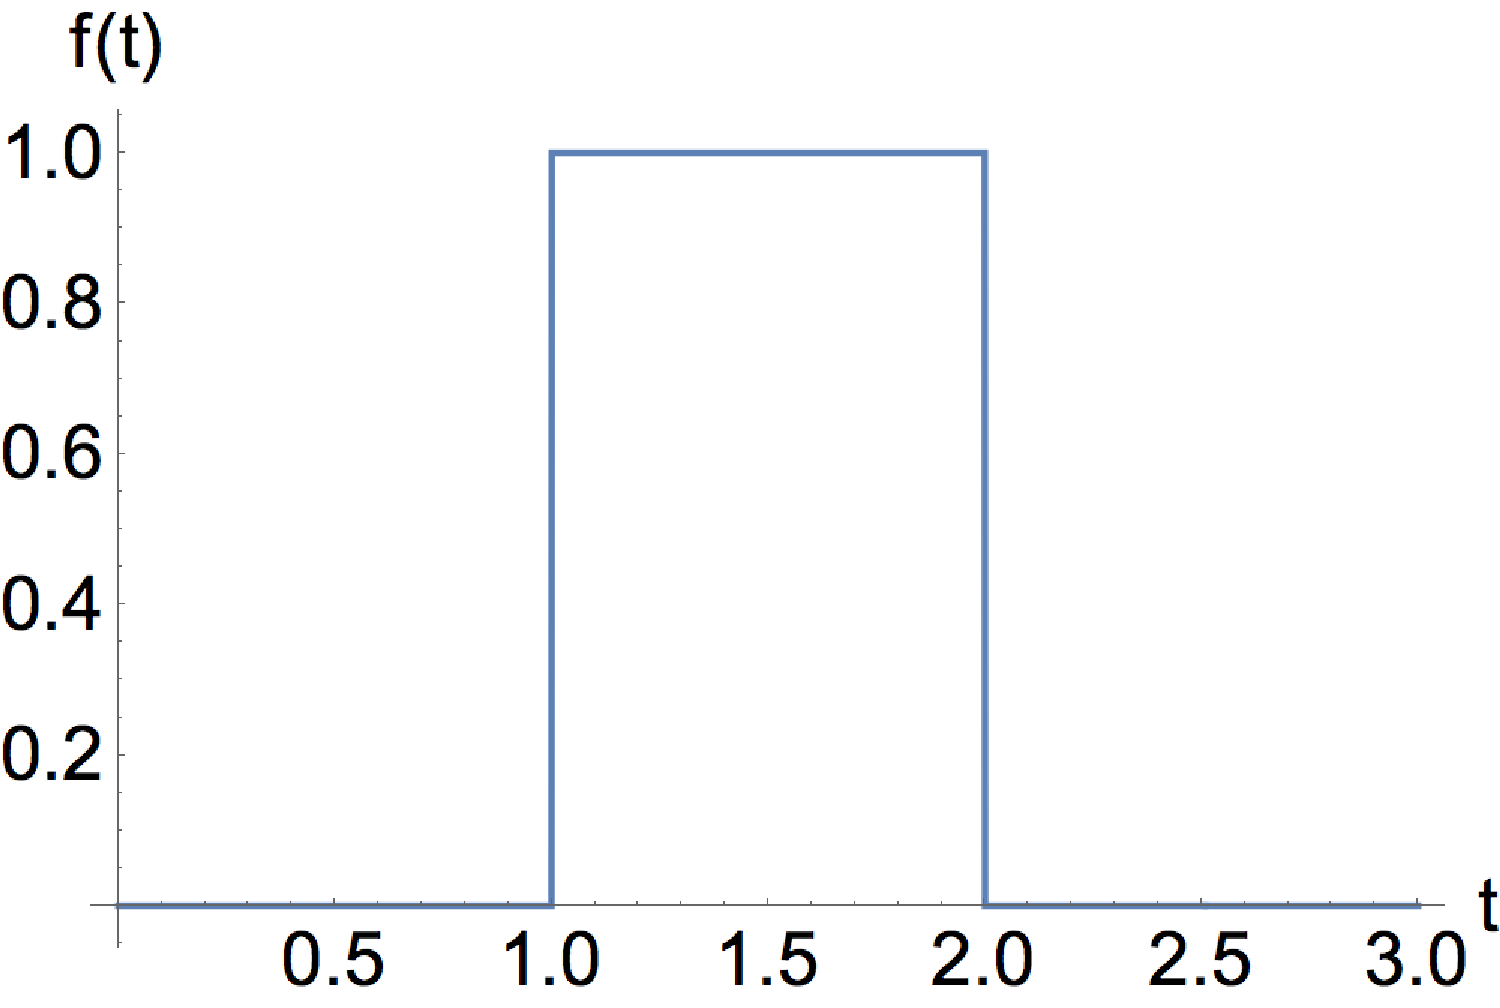
\includegraphics[scale=0.5]{pulse.png}

4. $\displaystyle \lap{U_\pi(t) cos(t-\pi)}$

\subsection*{Solution}
To check your answers, substitute $c=1$ and $s=2$ as appropriate.

1.\\
\soltwodp{y}{4f9ac8}

2.\\
0.0677

3.\\
0.0585

4.\\
\num{7.470e-4}




%%%%%%%%%%%%%%%%%%%%%%%%%%%%%%%%
\newpage
%%%%%%%%%%%%%%%%%%%%%%%%%%%%%%%%
\section{Inverse Laplace Transform}

\subsection*{Resources}
\begin{itemize}
    \item Video: \url{https://www.khanacademy.org/math/differential-equations/laplace-transform/properties-of-laplace-transform/v/inverse-laplace-examples} % 19m
\end{itemize}

\subsection*{Comment}
Being able to reversing the Laplace transform is a crucial skill required for applying it to solving ODE's. It can be a little confusing at first however, so I recommend to take your time to understand the essential steps involved thoroughly, as this will then give you greater confidence when you come to apply this to solving ODE's. To this end, the video listed in the resource is a fantastic introduction to this.

\subsection*{Challenge}
Determine the function $f(t)$ by finding the inverse of the following Laplace transforms:

1. $\displaystyle F(s)=\frac{1}{(s-1)^2}$

2. $\displaystyle F(s)=\frac{1}{s^2} - \frac{1}{s}$

%3. $\displaystyle F(s)=\frac{1-s}{s^2}$

3. $\displaystyle F(s)=\frac{5-5s}{s^2}$

4. $\displaystyle F(s)=\frac{6}{(2+s)^4}$

%5. $\displaystyle F(s)=\frac{120+6s^3}{s^6}$

5. $\displaystyle F(s)=\frac{2 e^{-2s}}{s^2-2s+2}$

6. $\displaystyle F(s)=\frac{e^{12-3s}}{s-4}$

\subsection*{Solution}
To check your answers, substitute $t=2$ into your final answer. If there is a unit-step in your solution, precede your numerical answer with ``u(c)'' where ``c'' is the position of the unit step. So for example, an answer of $U_5 t^2$ with a hash key of ``a'' would be entered as ``au(5.00)4.00'' (all numbers to two decimal places). An answer without a unit-step would just be entered to two decimal places (eg, ``a4.00'' in the previous example).

1.\\
\soltwodp{z}{de950a}

2.\\
\soltwodp{a}{a1e88c}

%3.\\
%\soltwodp{b}{1175d1}

3.\\
\soltwodp{c}{ae77f2}

4.\\
\soltwodp{c}{af01f2}

%5.\\
%\soltwodp{d}{d79888}

5.\\
\soltwodp{b}{b27f51}

6.\\
\soltwodp{e}{cbc74a}



\iffalse
%%%%%%%%%%%%%%%%%%%%%%%%%%%%%%%%
\newpage
%%%%%%%%%%%%%%%%%%%%%%%%%%%%%%%%
\section{The Dirac delta function and its Laplace transform}

\subsection*{Resources}
\begin{itemize}
    \item Video I: \url{https://www.khanacademy.org/math/differential-equations/laplace-transform/properties-of-laplace-transform/v/dirac-delta-function}
    \item Video II: \url{https://www.khanacademy.org/math/differential-equations/laplace-transform/properties-of-laplace-transform/v/laplace-transform-of-the-dirac-delta-function}
\end{itemize}

\subsection*{Challenge}
Calculate the following Laplace transforms (treat $c$ as a positive constant):

1. $\displaystyle \lap{\delta(t)}$

2. $\displaystyle \lap{\delta(t-c)}$

3. $\displaystyle \lap{\delta(t-2) Cos(4 t)}$

4. $\displaystyle \lap{\delta(t) (t^2+10)}$

\subsection*{Solution}
To check your solution, set $s=1$, $c=2$ and $t=1$ as appropriate to check your answers.

1.\\
\soltwodp{z}{a78955}

2.\\
\soltwodp{a}{ea59ed}

3.\\
\soltwodp{b}{48cb8f}

4.\\
\soltwodp{c}{c181ec}




%%%%%%%%%%%%%%%%%%%%%%%%%%%%%%%%
\newpage
%%%%%%%%%%%%%%%%%%%%%%%%%%%%%%%%
\section{The Dirac delta function and its inverse Laplace transform}

\subsection*{Challenge}
1. Calculate the following Laplace transform:

$\displaystyle \delta(t-2) Sin(2t)$

2. Calculate the following inverse Laplace transforms and state your answer in terms of the Dirac delta function:

I. $\displaystyle e^{-2s} Sin(2)$

II. $\displaystyle e^{-2s} Sin(4)$

\subsection*{Solution}
2. To check your answer, substitute $t=1$ into the final expression and evaluate the part inside and outside of the Dirac delta function separately. So for example, if your answer is $\delta(t-2) (t^2+1)$, the expression inside the delta-function is $t-2$ and will evaluate to $-1.00$ while the expression outside of the delta-function is $t^2+1$ and will evaluate to $2.00$.

I. Inside delta function:\\
\soltwodp{d}{4881ba}

I. Outside delta function\\
\soltwodp{e}{724c45}

II. Inside delta function:\\
\soltwodp{f}{75d06e}

II. Outside delta function:\\
\soltwodp{g}{fca71c}




%%%%%%%%%%%%%%%%%%%%%%%%%%%%%%%%
\newpage
%%%%%%%%%%%%%%%%%%%%%%%%%%%%%%%%
\section{A forced spring}

\begin{itemize}
    \item The \textbf{four} videos starting at \url{https://www.khanacademy.org/math/differential-equations/laplace-transform/laplace-transform-to-solve-differential-equation/v/laplace-transform-to-solve-an-equation}
    \item A useful table of Laplace transforms: \url{http://tutorial.math.lamar.edu/pdf/Laplace_Table.pdf}
\end{itemize}

\section*{Comment}
Here you finally get the opportunity to practise solving ODE's using the powerful method of Laplace transformations. Please takes notes from all four videos listed in the resources section; they provide very useful examples of how to use this method, including related algebraic techniques that are commonly required to solve such challenges.

\subsection*{Challenge}
The spring equation you encountered in challenge \ref{sec:hooke} introduced you to the concept of oscillation of a mass on a spring. There, the equation to determine the displacement of the spring $y$ from its equilibrium position was $y''+y=0$, which yields a solution $y=C_1 Cos(t) + C_2 Sin(t)$. This is free oscillation without external damping or driving, and it will oscillate according to the cosine and sine sum for all time ($t$). It is also possible to add a forcing term to the equation by making it non-homogeneous, such as in the form

\begin{equation}
    y'' + 4y = 2 Cos(3t)
\end{equation}

Here the forcing varies with time $t$ in the form of a cosine wave.

Use the Laplace transform method to solve the ODE in the above equation given a starting displacement of zero and an initial velocity of zero. You may use the table of Laplace transforms in the resources to help you.

\subsection*{Solution}
Substitute $t=1$ to check your final solution: $y(t=1)=0.2295$.




%%%%%%%%%%%%%%%%%%%%%%%%%%%%%%%%
\newpage
%%%%%%%%%%%%%%%%%%%%%%%%%%%%%%%%
\section{An exponential function}

\subsection*{Challenge}
Solve

\begin{equation}
    y''+5y'+4y=100e^{-2t}
\end{equation}

for $y$, given initial conditions $y(0)=-1$ and $y'(0)=0$. Since the algebra gets very messy, you may use the following equation to help you:
\begin{equation}
    \frac{-s^2-7s+90}{(s+1)(s+2)(s+4)} = \frac{32}{s+1} - \frac{50}{s+2} + \frac{17}{s+4}
\end{equation}

\subsection*{Solution}
Substitute $t=1$ to check your final solution: $y(1)=5.32$.




%%%%%%%%%%%%%%%%%%%%%%%%%%%%%%%%
\newpage
%%%%%%%%%%%%%%%%%%%%%%%%%%%%%%%%
\section{A unit step}

\subsection*{Comment}
In past challenges we studied the Laplace transform for $U_c f(t-c)$. So if $f(t)=t$ we must evaluate for $f(t-c)=t-c$. In the challenge here, we effectively have $f(t)=1$ and since ``1'' doesn't depend on $t$, $t-c$ doesn't do anything to the ``function''.

This challenge is interesting because unlike previous challenges, it is the first challenge where we really have no other option but to use the Laplace transform method, and so you can appreciate its power. In this challenge, we have a 2nd-order homogeneous equation (unforced oscillation) until $t=5$ when we apply a constant force. You will find your answer leads to a constant oscillation. But how can it lead to a constant oscillation if we are constantly applying a force? Shouldn't the oscillation slowly increase in magnitude due to the energy that is being added to the system from the constant force being applied? The answer is of course no: we take just as much energy out of the system when the velocity is in the opposite direction to the force as we add to the system when the velocity is in the same direction as the applied force.

One important point to note is that the inverse Laplace transform of $e^{-cs} s/(s^2+a^2)$ is $\lap{U_c Cos(a[t-c])}$ (not $\lap{U_c Cos([at-c])}$).

\subsection*{Challenge}
Solve

\begin{equation}
    y''+2y=U_5
\end{equation}

for $y$, given initial conditions $y(0)=0$ and $y'(0)=0$. 

\subsection*{Solution}

$y(t=6)=0.42$

Note that for $t<5$, the solution is zero. This is because there was no initial velocity and no initial acceleration, so there was no motion until a forcing was applied in terms of a constant force of ``1'' from $t=5$. If either of these had been non-zero, we would have had a non-zero value for $t<5$!

Optionally, you can try setting the initial conditions to non-zero values to see the effect this has on the final solution.




%%%%%%%%%%%%%%%%%%%%%%%%%%%%%%%%
\newpage
%%%%%%%%%%%%%%%%%%%%%%%%%%%%%%%%
\section{A sudden impulse}

\subsection*{Comment}
Here the system is stationary until $t=5$ when, instead of applying a constant force, we ``kick'' the system to start the oscillation. Thus you should expect your answer to reflect physics such as this.

\subsection*{Challenge}
Solve

\begin{equation}
    y''+2y=\delta(t-5)
\end{equation}

for $y$, given initial conditions $y(0)=0$ and $y'(0)=0$. 

\subsection*{Solution}

$y(6)=0.698$

Note how we have a simple oscillation after $t=5$, and nothing before it.
\fi
